\documentclass{article}

% Language setting
% Replace `english' with e.g. `spanish' to change the document language
\usepackage[english]{babel}

% Set page size and margins
% Replace `letterpaper' with `a4paper' for UK/EU standard size
\usepackage[letterpaper,top=2cm,bottom=2cm,left=3cm,right=3cm,marginparwidth=1.75cm]{geometry}

% Useful packages
\usepackage{amsmath}
\usepackage{amssymb}
\usepackage{graphicx}
\usepackage{parskip}
\usepackage[colorlinks=true, allcolors=blue]{hyperref}

\title{Multivariate linear regression by free energy minimization}
% \author{tianxun}

\begin{document}
\maketitle

\begin{abstract}
We provide an analytical solution for computing the entropy of multivariate linear regression, and use the results to propose a linear regression model that is fitted by optimizing the free energy, defined as the empirical loss minus weighted entropy.  
\end{abstract}

\section{Introduction}

In least squares linear regression, the regression model is fitted by finding the parameters that give the lowest empirical loss on training data. In low data situations, overfitting becomes a problem. Several regularization methods such as LASSO, ridge and elastic net are used to prevent overfitting through the introduction of penalty terms on the norm of the parameters in the loss function. In this work, inspired by statistical thermodynamics, we investigate a training scheme that minimizes the free energy instead of the empirical loss alone. Free energy is defined as 
\[
F = U - TS
\]
where $U$ is the empirical loss, $T$ the temperature, and $S$ the entropy. $S$ is a function of $U$. Entropy for a multivariate linear regression defined as a measure of the size of the solution space for a given empirical loss value.
The squared error loss function used in linear regression is convex and therefore has an unique solution at the minima. The unique minima therefore has the lowest possible entropy of this system. The solution space for loss values above the minima increases with increasing loss value. We are interested in an analytical formula for computing the size of the solution space, to be used as a measure of entropy.

\section{Analytical solution to compute entropy}
\subsection{Multivariate linear regression}
The general multivariate linear regression takes the following form:
\[
\hat{Y} = X\theta
\]

where $X \in \mathbb{R}^{m \times n}$ is the matrix of training data with $m$ being the number of datapoint, and $n$ being the number of features; $\theta \in \mathbb{R}^{n \times 1}$ is the vector of coefficients of the features; and $\hat{Y} \in \mathbb{R}^{m \times 1}$ is the vector of predicted value.

\par
The loss measured in squared error is thus
\[
\mathcal{L} = \sum_{i=1}^{m}(y_i - \hat{y_i})^2
\]
\[
\mathcal{L} = (X\theta-Y)^T(X\theta-Y)
\]
\[
\mathcal{L} = \theta^T X^T X\theta - 2Y^T X\theta + Y^T Y
\]
Note the shapes of the vectors and matrices:
\begin{itemize}
  \item $\theta^T X^T X\theta$ : $(1 \times n)\cdot(n \times m)\cdot(m \times n)\cdot(n \times 1)$
  \item $Y^T X\theta$ : $(1 \times m)\cdot(m \times n)\cdot(n \times 1)$
  \item $Y^T Y$ : scalar
\end{itemize}

\subsection{Entropy}
\subsubsection{Definition of entropy}
We define the entropy $S(u)$ as a measure of the size of the set of solutions when $\mathcal{L} = u$, where $u$ is some loss value. In other words, the size of the level set $L_u(\mathcal{L})$

\par
In 1-D case, where $n=1$, the number of solution for all valid $u > u_{min}$ is 2. For 2-D case, where $n=2$, there are infinite number of solutions for all valid $u > u_{min}$. Hence we choose to compute instead the circumference of the ellipse where the solutions lie on. In general, for $n$-D cases, we are interested in computing the surface area of the hyper-ellipsoid in $(n-1)$-D where the solutions lie upon.

\par
To compute the entropy from the circumference or surface area, we need to fix the size of the parameter space. The entropy may be defined as
\[
S(u) = ln(s(u)/V)
\]
where $s(u)$ is the surface area of the solution ellipsoid, and $V$ is the volume of the parameter space.
The minimum entropy correspond to the point of a single solution, $s(u) = 0$, which results in $S(u) \rightarrow -\infty$. This is not useful if the entropy is used later in free energy minimization. A possible work-around is using change in entropy instead,
\[
\Delta S = ln(s(u')/s(u))
\]
where $\Delta S$ is the change in entropy when $\mathcal{L}$ goes from $u$ to $u'$.

\subsubsection{Equation of solution}
The loss function for fitting a linear regression model, parameterized by $\theta$ to training data $X$, $y$ as defined previously is
\[
\mathcal{L} = \theta^T X^T X\theta - 2Y^T X\theta + Y^T Y
\]
We would like to find the equation of the hyper-ellipsoid where $\mathcal{L} = u$ s.t. $u > u_{min}$. i.e.

\[
f = \theta^T X^T X\theta - 2Y^T X\theta + Y^T Y - u = 0
\]

Let $A = X^T X$, $b = -2Y^T X$ and $c = Y^T Y - u$,
\[
f = \theta^T A\theta + b\theta + c = 0
\]

This is equivalent to the matrix representation of a hyper-conic. The equation represents a hyper-ellipsoid iif $det(A) > 0$. As $A$ is defined to be $X^T X$ which is positive semidefinite, thus $det(A) \geq 0$. $det(A)$ may be $0$ if any 2 or more columns of $X$ are linearly dependent, which means the dimension would be reduced. The minima or center of $f$, $\theta_c$ and the corresponding $f$ value, $u_{min}$ is obtained by taking derivative of $f$ with respect to $\theta$ and equating to $0$,

\[
\theta_c^T = -\frac{1}{2}bA^{-1}
\]

$f$ can be re-written with this center as such
\[
(\theta - \theta_c)^T A (\theta - \theta_c) = \theta^T A \theta - 2\theta^T A \theta_c + \theta_0^T A \theta_0
\]
\[
= \theta^T A \theta + b\theta + \theta_0^T A \theta_0
\]
\[
= \theta_c^T A \theta_c - c
\]

$A$ can be diagonalized using eigendecomposition into 
\[
A = Q\Lambda Q^{-1}
\]
where $Q$ is the square $n \times n$ matrix whose ith column is the eigenvector $q_i$ of $A$, and $\Lambda$ is the diagonal matrix whose diagonal elements are the corresponding eigenvalues $\lambda_i$. The eigenvectors of $A$ are the principle axes of the hyper-ellipsoid, and therefore orthogonal to each other, hence $Q^{-1} = Q^T$ and we can write $A$ as $Q \Lambda Q^{T}$.

Substituting this into $f$,
\[
(\theta - \theta_c)^T Q\Lambda Q^T (\theta - \theta_c) = \theta_c^T A \theta_c - c
\]

Let $K=\frac{\Lambda}{\theta_c^T A \theta_c - c}$ and $v = Q^T(\theta - \theta_c)$, then we obtain the canonical form of the hyper-ellipsoid.

\[
v^T K v = 1
\]

The diagonal entries of the matrix $K$ are the reciprocal of the ellipsoid principal axes length, $a$ squared, i.e.

\[
K = \begin{bmatrix} \dfrac{1}{a_1^2} && 0 && \dots && 0 \\0 && \dfrac{1}{a_2^2} && \dots && 0 \\ \vdots && \vdots && \ddots && \vdots \\ 0 && 0 && \dots && \dfrac{1}{a_n}^2 \end{bmatrix}
\]

\subsubsection{Entropy of 2-D case}
% We examine the 2-D case below:
% \[
% \mathcal{L} = 
% \begin{pmatrix} \theta_1 & \theta_2 \end{pmatrix}
% X^T X
% \begin{pmatrix} \theta_1\\ \theta_2 \end{pmatrix}
% - 2Y^T X
% \begin{pmatrix} \theta_1\\ \theta_2 \end{pmatrix}
% + Y^T Y = u
% \]
% This is equivalent to the matrix representation of a conic section satisfy a second-degree polynomial equation in two variables.

% \[
% f(\theta_1, \theta_2) = A\theta_1^2 + B\theta_1 \theta_2 + C \theta_2^2 + D\theta_1 + E\theta_2 + F = 0
% \]
% \[
% f =
% \begin{pmatrix} \theta_1 & \theta_2 \end{pmatrix}
% \begin{pmatrix} A & B/2\\ B/2 & C \end{pmatrix}
% \begin{pmatrix} \theta_1\\ \theta_2 \end{pmatrix}
% + 
% \begin{pmatrix} D & E \end{pmatrix}
% \begin{pmatrix} \theta_1\\ \theta_2 \end{pmatrix}
% + F = 0
% \]
% Let $A_{33} = X^T X = \begin{pmatrix} A & B/2\\ B/2 & C \end{pmatrix}$, $\begin{pmatrix} D & E \end{pmatrix} = -2Y^T X$ and $F = Y^T Y - u$.

% \par
% The quadratic equation can also be rewritten using homogeneous coordinate vector as $\Theta^T A_Q \Theta = 0$ where $\Theta = \begin{pmatrix} \theta_1 & \theta_2 & 1\end{pmatrix}^T$
% \[
% A_Q = 
% \begin{pmatrix}
% A & B/2 & D/2\\
% B/2 & C & E/2 \\
% D/2 & E/2 & F
% \end{pmatrix}
% \]

% \par
% The equation represents an ellipse iif $det(A_{33}) > 0$. As $A_{33}$ is defined to be $X^T X$ which is positive semidefinite, thus $det(A_{33}) \geq 0$. $det(A_{33})$ may be $0$ if $AC = B^2/4$. This may occur if the 2 columns of $X$ are linearly dependent, which means the dimension is reduced to 1-D, and the equation becomes a parabola instead of an ellipse. The minima of $\mathcal{L}$, $u_{min}$ is obtained by taking derivative of $\mathcal{L}$ with respect to $\theta$ and equating to $0$,
% \[
% \theta_c=(X^TX)^{-1} X^T Y
% \]
% \[
% \theta_c=A_{33}^{-1} \begin{pmatrix} -D/2\\ -E/2 \end{pmatrix}
% \]
% When the $\theta = \theta_c$, $det(A_Q)=0$, which indicate a degenerate conic, i.e. a single point.
% With this, we know that given proper input $X$ that is has linearly independent columns, for any $\mathcal{L} > u_{min}$, the solution lies upon an ellipse.

% \par
% We can now compute the characteristics of the ellipse. The center of the ellipse is the same point as the minima, i.e.
% \[
% \begin{pmatrix} \theta_{1, c}\\ \theta_{2, c} \end{pmatrix}
% = A_{33}^{-1}
% \begin{pmatrix} -D/2\\ -E/2 \end{pmatrix}
% \]

% \par
% The ellipse can be obtained when a centered ellipse with the same axis lengths is translated to $\begin{pmatrix} \theta_{1, c} & \theta_{2, c} \end{pmatrix}^T$ and then rotated by an angle. The rotation can be carried out by diagonalizing the matrix $A_{33}$. We can write the equation of the centered ellipse as
% \[
% \lambda_1 \theta_1^2 + \lambda_2 \theta_2^2 = -\frac{det (A_Q)}{det (A_{33})}
% \]
% \[
% \frac{\theta_1^2}{K/\lambda_1} + \frac{\theta_2^2}{K/\lambda_2} = 1
% \]
% where $\lambda_1$ and $\lambda_1$ are the eigenvalues of $A_{33}$.
% The lengths of the major $a$ and minor axis $b$ are $\sqrt{K/\lambda_1}$ and $\sqrt{K/\lambda_2}$ respectively

% \par
In the $2$-D case, we want to compute the circumference of the solution ellipse with principal axes $a$ and $b$. The circumference $C$ of an ellipse is 
\[
C = 4a \int_{\phi=0}^{\pi/2} \sqrt{1-e^2sin^2\phi}\ d\phi
\]
where $e=\sqrt{1-b^2/a^2}$, and can be computed using Gauss's arithmetic-geometric mean method, which is a quadratically converging iterative method.

% Alternatively, we can also approximate using a Ramanujan approximation, 
% \[
% C \approx \pi (a+b)\left(1+\frac{3h}{10+\sqrt{4-3h}}\right)
% \]
% where $h=(a-b)^2/(a+b)^2$, with an error on the order of $h^5$.

Notice that as $u$ increases, the ratio between the axes stays constant, therefore, $e$ remains constant and $C$ scales linearly with the $a$, which scales in a square root relationship with $u$:
\[
\frac{1}{a_i^2} = \frac{\lambda_i}{\theta_c^T A \theta_c - Y^TY + u}
\]
\[
a \propto \sqrt{u} \implies C \propto \sqrt{u}
\]
The entropy is $S = ln(C(a, b)/V)$. We illustrate the trend of unnormalized $S$ with respect to $u$ in Fig. \ref{S_against_u} for some arbitrary data.

\begin{figure}[!h]%
\centering
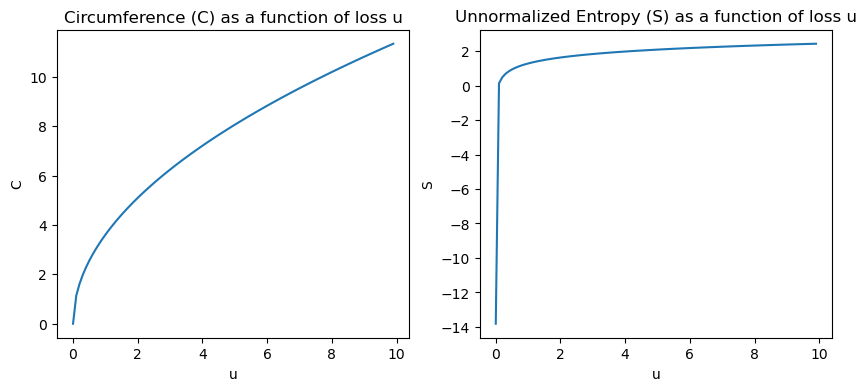
\includegraphics[width=0.9\textwidth]{figures/S_against_u.png}
\caption{\textbf{a.} Plot of circumference $C$ against empirical loss $u$; \textbf{b.} Plot of entropy $S$ against empirical loss $u$}\label{S_against_u}
\end{figure}

\subsubsection{Entropy of n-D case}
To find the surface area of a $n$-D hyper-ellipsoid, we use an approximation formula given by [Knud Thomson (\url{http://www.numericana.com/answer/ellipsoid.htm#thomsen})] that makes use of the generalized mean (Hölder mean), $H$ of the $n$ products of $n-1$  axes
\[
s \approx \frac{2\pi^{n/2}H}{\Gamma(n/2)}
\]
where,  
\[
H =\left(\frac{1}{n} \sum_{i=1}^n \prod_{j \neq i}^n a_j \right)^{\frac{1}{p}} = \left((a_1 a_2 ... a_n)^p \left(\frac{a_1^{-p} + a_2^{-p} + ... + a_n^{-p}}{n} \right)\right)^{\frac{1}{p}}
\]
\[
p = \frac{log(n)}{log(D)}
\]
\[
D = 
\begin{cases}
  (\pi/2)(n-1)!!/(n-2)!! & \text{if}\ n=2k \\
  (n-1)!!/(n-2)!! & \text{if}\ n=2k+1
\end{cases}
\]
$n!!$ is the product of all the positive integers up to n that have the same parity (odd or even).

Again, as the ratio between axes stays constant, $H$ scales with any axes length $a$ as
\[
H \propto a^{n-1}
\]
\[
a \propto \sqrt{u} \implies s \propto u^{(n-1)/2}
\]

\section{Minimization of free energy}
\subsection{Loss function}
The loss function to minimize is
\[
\mathcal{L}_{FE} = U - TS
\]
\[
\mathcal{L}_{FE} = U - T\alpha ln\left(U^{(n-1)/2}\right)
\]
% \[
% \mathcal{L} = \frac{1}{m}\sum_{i=1}^{m}(y_i - \hat{y_i})^2 - T\alpha\left(\sum_{i=1}^{m}(y_i - \hat{y_i})^2\right)^{(n-1)/2}
% \]
where $\alpha$ is some constant term.

To minimize this new loss function, we take derivative of $\mathcal{L}_{FE}$ with respect to $U$ and equate to 0. $U*$ is required to be larger than or equal to $u_{min}$. 
\[
\frac{d\mathcal{L}_{FE}}{dU} = 1 - \frac{T\alpha(n-1)}{2U} = 0
\]
% \[
% U^* = max\left(u_{min}, \left(\frac{T\alpha(n-1)}{2}\right) \right)
% \]
\[
U^* = \frac{T\alpha(n-1)}{2}, \; \text{where } T \geq \frac{2u_{min}}{\alpha (n-1)}
\]

Substituting $U^*$ into the hyper-ellipsoid equation, the solutions that minimize our new loss function $\mathcal{L}_{FE}$ satisfies the following equation
\[
\theta^T X^T X\theta - 2Y^T X\theta + Y^T Y - U^* = 0
\]

\subsection{Parameter sampling and inference}
As infinite sets of parameters exist that satisfies the above equation, we may chose to sample $M$ sets of parameters and ensemble the predictions of all $M$ regression models as the final prediction.

To sample parameters from the $n$-D solution space, we can first generate random samples on a $n-D$ hyper-sphere. The points are then linear transformed to lie on the hyper-ellipse. To ensure even sampling occurs on the hyper-ellipse, rejection sampling is applied based on the amount of change in surface area around the point after transformation to hyper-ellipsoid.

We now have a set of sampled parameters $\theta_{M} \in \mathbb{R}^{n \times M}$. 

\subsubsection{Ensembling models for inference}
During inference, we can compute the predictions of each of these $M$ models,
\[
\hat{Y}_M = X\theta_{M}
\]
The predictions can be ensembled by various ways. For example, taking the mean prediction of the $M$ models
\[
\hat{Y} = \frac{1}{M}\sum_{i=1}^M col_i(\hat{Y}_M)
\]

To improve upon the naive method of mean ensembling, we propose a model weighting scheme to ensemble the models based on some measure of model quality. We may choose to measure the model quality based on certain inductive biases. Here we list 3 possible ways to define the model quality, $q$

\begin{itemize}
  \item Model parameter norm, such as $L_2$ or $L_1$ norm. E.g. $q=||x||_2$
  \item Norm of model derivative, or magnitude of local gradient at inference location. E.g. $q=||\frac{\delta \hat{Y}}{\delta \theta}(x_i)||_2$, where $x_i$ is the inference location and $\hat{Y}$ is the prediction by the model
  \item Variance of prediction for some random sample of inputs, or at neighborhood around inference location. E.g. $q = \sigma^2(\hat{Y}_{i,1}, \hat{Y}_{i,2} ... \hat{Y}_{i,})$ where $\hat{Y}_{i,j} = x_{i,j}\theta$, and $x_{i,j} = x_i + \varepsilon$, for some $\varepsilon$ such that $x_{i,j}$ is in a small neighborhood around $x_i$
\end{itemize}

The weighting, $w$ of the models can be computed using a negatively correlated function with quality. For example, $w=1/q$.

\section{Under-determined systems}
In section 2, we have assumed that the linear system is well determined, i.e. $m \geq n$. However in cases, we may have an under-determined system where $m < n$. Other cases occur when $m \geq n$ but some columns of $m$ are linearly dependent, which results in a matrix rank $< n$. The under-determined system is dealt with in this section.

\subsection{Least norm solution}
In an under-determined system, there are infinite solutions for $\theta$. One particular solution is the least norm solution, $\theta_{ln}$, and can be found by
\[
Y = X\theta
\]
\[
\theta_{ln} = X^T (X X^T)^{-1} Y
\]
\[
\theta_{ln} = X^{\dag} Y
\]
$X_{\dag}$ is the pseudo-inverse of $X$. 
As $\theta_{ln}$ is the least norm solution, it is necessarily orthogonal to solution space.

\subsection{Geometry of solution set and loss function}
The set of solutions of a linear system $X\theta = Y$ where $X \in \mathbb{R}^{m \times n}$ has dimensions equal to the degrees of freedom (DOF) $n-m$ assuming the $X$ is full ranked. Concretely, this means that the solution is unique point when $\text{DOF}=0$, a line when $\text{DOF}=1$, a plane when $\text{DOF}=2$ and a $n$-D hyperplane for $\text{DOF} > 2$.

The loss function with its minima centered at any particular solution, and direction of the function domain orthogonal to, or at least not lying on the solution space (because staying in the solution space means the loss is always 0, and therefore there is no meaningful loss function to speak of), is a $m$-D paraboloid. The level set $L_u(\mathcal{L})$, which we are interested in for calculating entropy is a $m$-D ellipsoid. 

To illustrate with an example, let us consider a linear system where $n=3$:
\begin{itemize}
\item If $m=2$, the $\text{DOF}=1$, which means that the solution lies on a line. If we choose a particular solution on this line, for e.g. fix one parameter (since \text{DOF} is 1) to be $0$ and plot the loss function with respect to the remaining two parameters, we will obtain a $2$-D paraboloid with the minima with a value of $0$ centered at the the chosen particular solution. The level set for any $u > 0$ is an ellipse. 

\item If $m=1$, the $\text{DOF}=2$, which means that the solution lies on a plane. If we choose a particular solution on this plane, for e.g. fix two parameter to be $0$ and plot the loss function with respect to the remaining one parameter, we will obtain a parabola with the minima with a value of $0$ centered at the the chosen particular solution. The level set for any $u > 0$ is an "$1$-D ellipse", which is degenerate and in this case is just a set of two points on the parabola at the $u$.
\end{itemize}

\subsection{Parameter sampling}
Out of the infinite solutions and thus infinite loss functions and levels sets to sample the model parameters from, a reasonable choice would be to use the loss function centered at the least norm solution $\theta_{ln}$. To define the $m$-D paraboloid loss function at that point, we would require $m$ vectors that will make up the new basis for the loss function. The vectors would need to be orthogonal; they would need to not lie on the solution space. 

$\theta_{ln}$ itself is orthogonal to the solution space, so it satisfies as the one of the basis vectors. The remaining $m-1$ vectors can be can be any vectors orthogonal to both each other and to the solution space. We can iteratively obtain these $m$ orthogonal vectors, $v_1, v_2 ... v_m$ by following the algorithm given in the appendix. 

We can now transform the original loss function $\mathcal{L}$ into a new loss function parameterized by a $m$-D $\Theta$ in the new basis $V$, where $\theta = V\Theta$
\[
V = 
\begin{bmatrix}
 \vdots & \vdots & \vdots & \vdots\\
 v_1 & v_2 & ... & v_m\\
 \vdots & \vdots & \vdots & \vdots
\end{bmatrix}
\]

\[
\mathcal{L} = \theta^T A\theta + b\theta + c = 0
\]
\[
\mathcal{L} = \Theta^T V^T A V \Theta + bV\Theta + c = 0
\]
\[
\mathcal{L} = \Theta^T A^{'} \Theta + b^{'}\Theta + c = 0
\]
where $A^{'} = V^T A V$ and $b^{'} = bV$

Note the shapes of the vectors and matrices:
\begin{itemize}
  \item $\Theta$ : $(m \times 1)$
  \item $V$ : $(n \times m)$
  \item $A = X^TX$ : $(n \times m)\cdot(m \times n) = (n \times n)$
  \item $\Theta^T V^T A V \Theta$ : $(1 \times m)\cdot(m \times n)\cdot(n \times n)\cdot(n \times m)\cdot(m \times 1)$
  \item $b = -2Y^TX$ : $(1 \times m)\cdot(m \times n) = (1 \times n)$
  \item $bV\Theta$ : $(1 \times n)\cdot(n \times m)\cdot(m \times 1)$
\end{itemize}

With this loss function (equation of hyper-ellipsoid) $\mathcal{L} = \Theta^T A^{'} \Theta + b^{'}\Theta + c = 0$, we can use the same ellipsoid sampling technique as described in section 3.2 to sample for $\Theta$. $\Theta$ is then converted back to $\theta$ with $\theta = V\Theta$.

\bibliographystyle{alpha}
\bibliography{sample}

\section*{Appendix}

\textbf{Algorithm}: for finding $m$ orthogonal vectors, none of which lies on the solution space of $X\theta = Y$.
\begin{enumerate}
  \item Find vector(s) that lie on the solution space which are the columns of the nullspace (kernel) of $X$, $\textbf{Ker}(X)$
  \item Let $v_1 = \theta_{ln}$
  \item Find an orthogonal vector to both the columns of $\textbf{Ker}(X)$ and all $v_i$ using cross product (generalized to $n$-D). Perform cross product between all the columns of $\textbf{Ker}(X)$ and $v_{i}$.
  \begin{enumerate}
     \item Cross product in $n$-D is only valid between $(n-1)$ vectors. The number of columns of $\textbf{Ker}(X)$ is equal to the DOF. This means that we have at the beginning $\text{DOF} + 1$ vectors available. If $\text{DOF} + 1 < n - 1$, we are unable to perform the cross product 
     \item To resolve this, consider a matrix where the columns are composed of orthogonal vectors. We can partition the matrix such that the number of rows $=$ number of columns $+ 1$. The top partitioned matrix, $v_{top}$ now contains the correct dimension and number of vectors to perform cross product. The resulting vector concatenated with correct number of $0$s is now a new orthogonal vector.
  \end{enumerate}
    \[
        \left[ 
        \begin{array}{cccc} 
         \vdots & \vdots & \vdots & \vdots\\
         %\textbf{Ker}(X) & v_1 & v_2 & ...\\
         v_1 & v_2 & ... & v_i\\
         \vdots & \vdots & \vdots & \vdots\\
         \hline 
         : & : & : & : \\
        \end{array}
        \right] 
    =
        \left[ 
        \begin{array}{c} 
          v_{top}\\ 
          \hline 
          v_{bot} 
        \end{array} 
        \right] 
    \]
    \[
    v_{i+1, top} = v_{1, top} \times v_{2, top} \times ... \times v_{i, top}
    \]
    \[
    v_{i+1} = 
        \left[ 
        \begin{array}{c} 
          \vdots \\
          v_{top}\\ 
          \vdots \\
          \hline
          :\\
          0\\
          : 
        \end{array} 
        \right] 
    \]
  \item repeat the step above until $m$ orthogonal vectors, $v_1, v_2 ... v_m$ are obtained.
\end{enumerate}
\end{document}

    % =
    %     \left[ 
    %     \begin{array}{c|c} 
    %       K_{1:m+1} & v_{1:m+1}\\ 
    %       \hline 
    %       K_{m+2:n} & v_{m+2:n} 
    %     \end{array} 
    %     \right] 
    % =